\chapter{Grundlagen} \label{basics}
Wie bereits oben erwähnt, wird für diese Arbeit ein geeignetes Speicherformat für 3D Modelle von Gebäuden benötigt.
Um den Bau von Gebäuden zu automatisieren, ist es notwendig die Domäne \textit{Gebäude} vollständig digital abbilden zu können. 
Hilfreich ist dabei, wichtige Daten über bestimmte Bestandteile des Gebäudes direkt in das Modell zu integrieren auf Basis derer etwa Kostenberechnungen durchgeführt oder Materialmengen herausgefunden werden können.
Da diese oft von verschiedenen Experten vieler Fachbereiche (etwa aus den Bereichen der Architektur, des Bauwesens oder der Statik) stammen, muss das Format sehr flexibel und im besten Fall auch zeitgleich bearbeitbar sein.
Dafür werden seit 2000 die \textit{Industry Foundation Classes} (IFC) von buildingsmart entwickelt, deren Anwendung im internationalen Bauwesen mittlerweile weit verbreitet ist \cite{Industry61:online}.


\section{Industry Foundation Classes}
\label{basics:ifc}
%Kurze Einleitung was IFC ist
In der Spezifikation des Standards selbst, wird dieser wie folgt beschrieben:
"Die Industry Foundation Classes (IFC) sind ein offener internationaler Standard für Daten des Building Information Model (BIM), welche zwischen Softwareanwendungen ausgetauscht, gemeinsam genutzt und von den verschiedenen Akteuren der Bauindustrie und des Gebäudemanagements verwendet werden. 
Der Standard enthält Definitionen für Daten, die für die Lebenszyklen von Gebäude- und Infrastrukturarbeiten erforderlich sind. 
Die bis jetzt in die IFC aufgenommenen Infrastrukturtypen umfassen Brücken, Straßen, Eisenbahnen, Wasserstraßen und Hafenanlagen" (aus dem Englischen) \cite{IFCScope:online}. 
Eine frühere Version des IFC Standards ist unter der Bezeichnung ISO 16739\cite{ISOISO1694:online} registriert.
Da die IFC aber nach wie vor kontinuierlich weiterentwickelt werden, wird in dieser Arbeit die derzeit neueste Version verwendet.
Diese ist die IFC Spezifikation 4.3.1.0 \cite{IFC4310Spezification:online}.
Das verbreitetste Austauschformat für IFC ist das Step Physical File Format, welches im ISO 10303 Teil 21 registriert ist \cite{ISO_Step:online}.
Zudem gibt es speicherreduziertere Formate wie ifcZip oder für Menschen lesbarere Formate wie ifcXML \cite{Industry93:online} \cite{IFCForma28:online}.

\subsection{IFC 4.3.1.0 Aufbau}
Im Grunde definieren die \textit{Industry Foundation Classes} eine Vielzahl an Klassen, die in einer komplexen Hierarchie angeordnet den Grundstock des Datenmodells bilden.
Diese sind anfangs abstrakte Konzepte, die sich mit zunehmender Tiefe in der Hierarche konkretisieren.

\begin{figure}[ht]
    \centering
    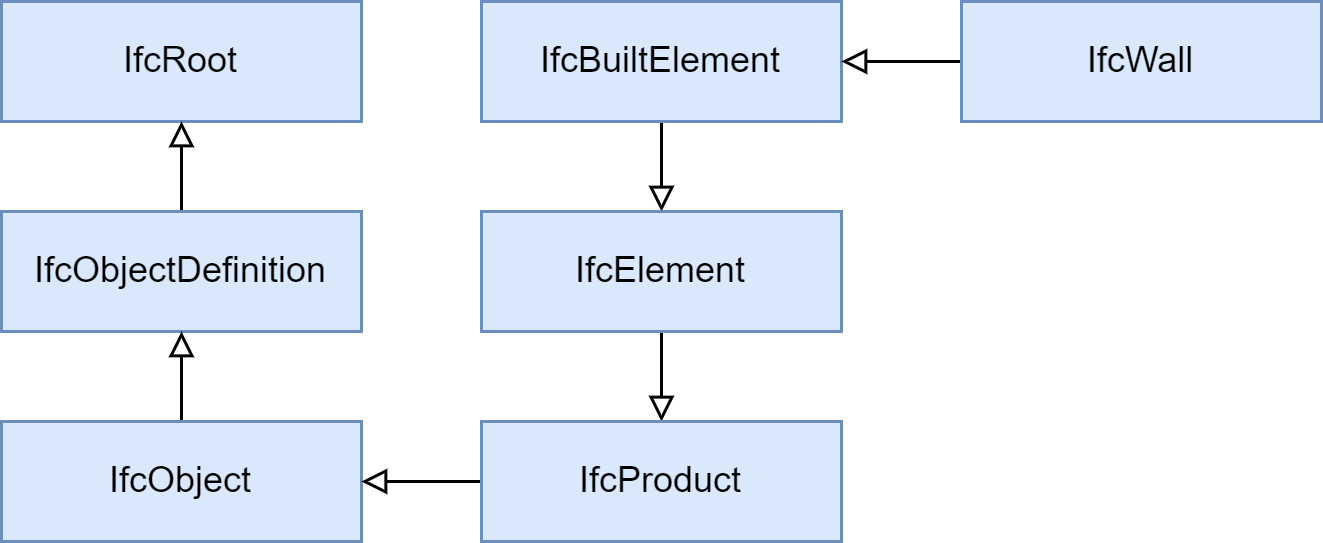
\includegraphics[width=0.6\columnwidth]{fig/Hierarchie_IfcWall_300.drawio.png}
    \caption{Klassenhierarchie am Beispiel der Klasse \textit{IfcWall}}
    \label{fig:IfcWall_Hierarchie}
\end{figure}

Da sich diese Arbeit zum größten Teil mit aus Wänden bestehenden Gebäuden befasst, wird nachfolgend die Klasse \textit{IfcWall} wiederholt als Beispiel herangezogen.
Der für diese Klasse relevante Ausschnitt aus der Klassenhierarchie ist in Abbildung \ref{fig:IfcWall_Hierarchie} dargestellt.
Objekte werden von dem Standard in Relation zueinander gestellt, um komplexere Zusammenhänge darzustellen.
In Abbildung \ref{fig:IFC_Relationships} erkennt man den Zusammenhang zwischen einem Objekt des Types \textit{IfcWall}, des Stockerwerks, welches diese Wand referenziert und wiederum selbst Teil eines \textit{IfcBuildings} ist, bis hin zur obersten Komponente eines Ifc Projektes, dem gleichnamigen \textit{IfcProject}.

\begin{figure}[h]
    \centering
    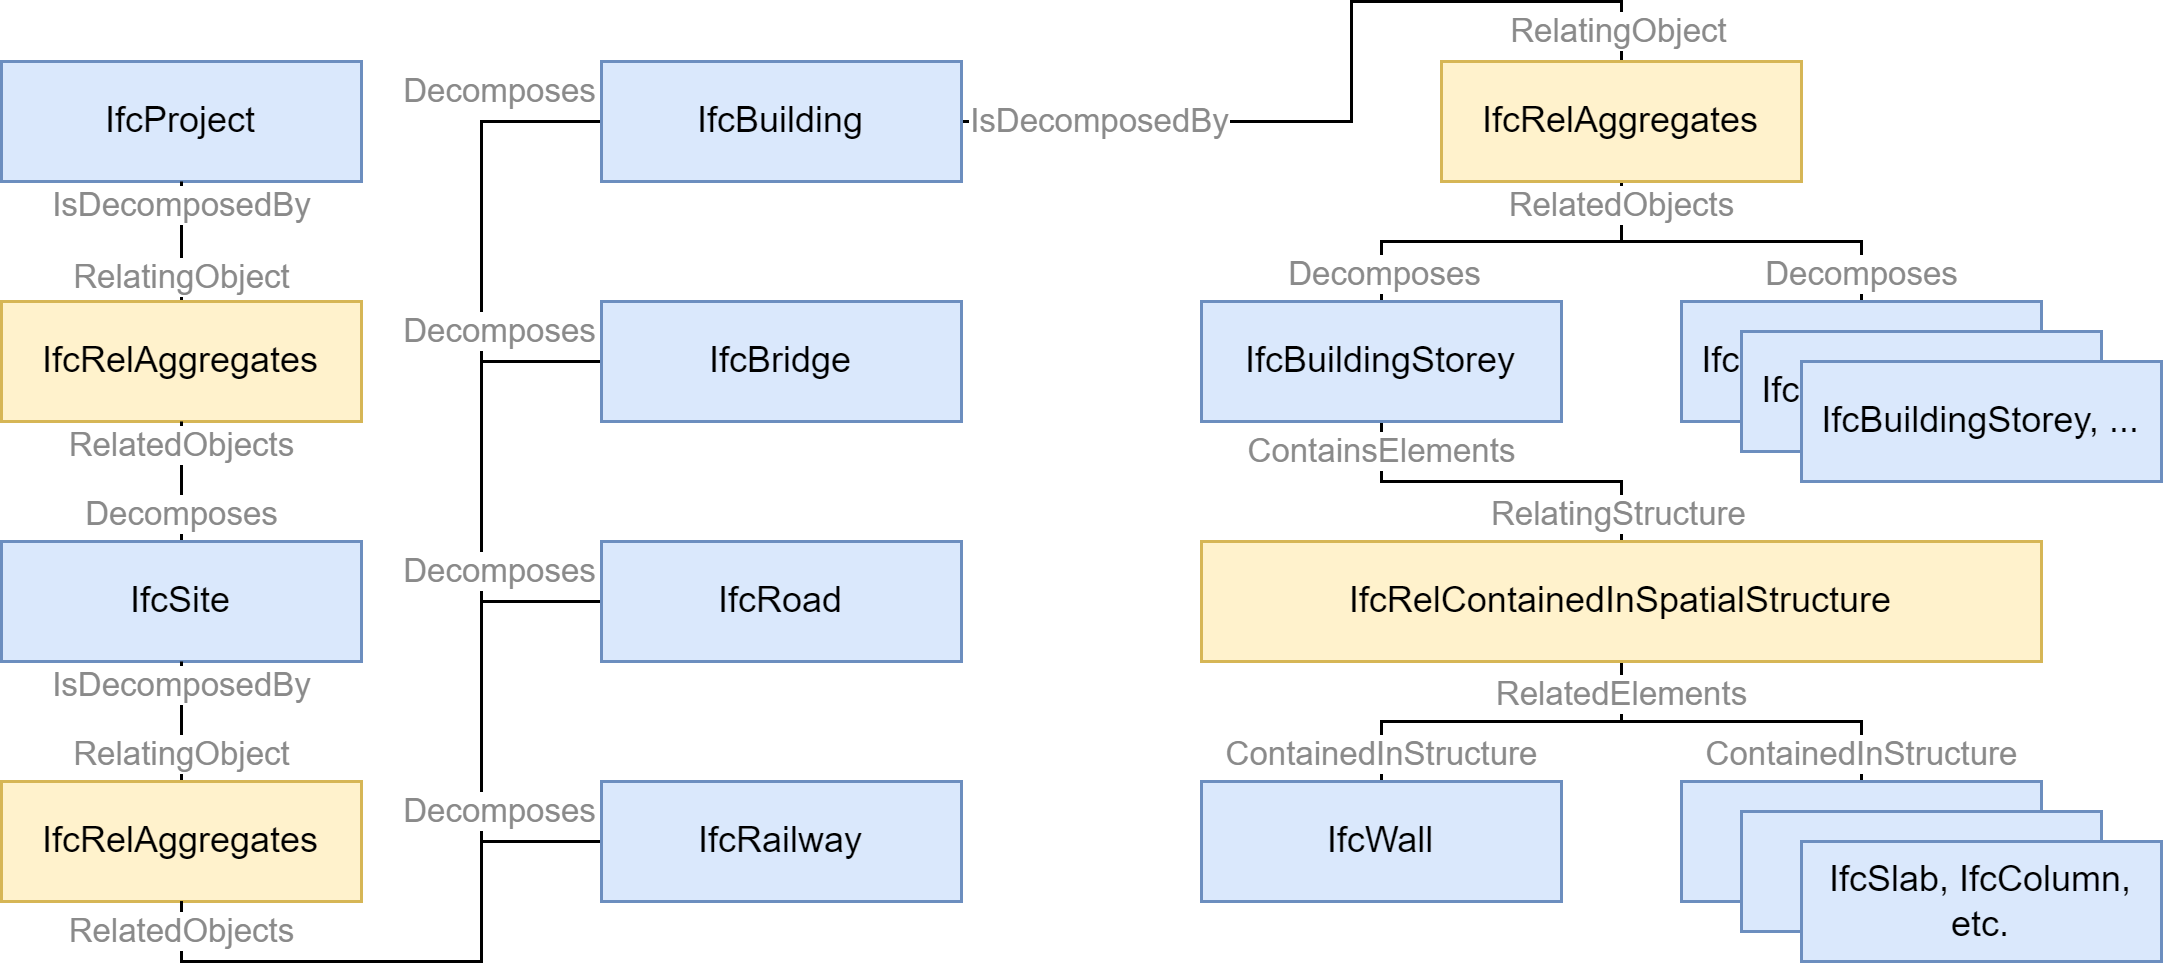
\includegraphics[width=0.9\columnwidth]{fig/IFC_Relationships_300.drawio.png}
    \caption{Relation der IfcWall und einem IfcProjekt}
    \label{fig:IFC_Relationships}
\end{figure}

\subsection{IfcPropertySets und IfcQuantitySets}
Mit dem Erweitern des Gebäudemodells um möglichst viele Informationen, schafft man einen detailierten digitalen Zwilling, der neben der bloßen Darstellung des Gebäudes als 3D Modell zb. auch eine präzisere Kosten- und Zeitschätzung für den Bau ermöglicht \cite{Industry93:online}. 
Dies kann mithilfe der IfcPropertySets und der IfcQuantitySets umgesetzt werden blablabla. %TODO
%TODO diagramm, beispiel Properties und Quantities

\subsection{Positionierung von IFCProducts}
%https://ifc43-docs.standards.buildingsmart.org/IFC/RELEASE/IFC4x3/HTML/concepts/Product_Shape/Product_Placement/Product_Local_Placement/content.html
TODO: Positionierung ist anscheinend bisschen verschachtelt
Blablabla so können aus einem IFC Projekt alle relevanten Klassen mit den für diese Arbeit erforderlichen Eigenschaften extrahiert werden.


\subsection{IfcOpeningElement}
\label{basics:IfcOpeningElement}
Wie funktionieren Löcher in z.B. IfcWall? -> IfcOpeningElement.
Am Beispiel eines Fensters erklären. In dessen Doku steht dass Windows auf ein IfcOpeningElement verweisen, welches ein Stück Wand wegmacht und z.b. durch das Fenster aufgefüllt wird.
%(https://ifc43-docs.standards.buildingsmart.org/IFC/RELEASE/IFC4x3/HTML/lexical/IfcWindow.htm) 
%https://standards.buildingsmart.org/IFC/DEV/IFC4_2/FINAL/HTML/schema/ifcproductextension/lexical/ifcopeningelement.htm
TODO: mit rausparsen und aus wandmeshes rauschneiden vor detailing.

ifcopeningelement um lücken in wände zu machen.
"The opening element stands for opening, recess or chase, all reflecting voids. It represents a void within any element that has physical manifestation. Openings can be inserted into walls, slabs, beams, columns, or other elements." Auszug aus Doku. und This also includes IfcOpeningElements, the mechanism used to extract openings for windows and doors, typically from walls. %https://academy.ifcopenshell.org/posts/using-ifcopenshell-and-pythonocc-to-construct-new-geometry/
%https://ifc43-docs.standards.buildingsmart.org/IFC/RELEASE/IFC4x3/HTML/lexical/IfcDoor.htm

\section{IFC for Blender}
\subsection{Blender}
Blender ist eines der beliebtesten Open Source Programme zur Modellierung von 3D Modellen und Animationen \cite{blendero56:online}.
Aufgrund dessen existieren auch eine Vielzahl an freien Erweiterungen bzw. Plugins - unter anderem auch eine Integration von IFC Projekten.

\subsection{blenderbim}
Neben kommerziellen Produkten wie etwa revit von autodesk \cite{RevitSof26:online} zur Modellierung von IFC Modellen, gibt es auch für Blender ein freies Plugin, um IFC Modelle zu erstellen \cite{BlenderB43:online}.
Dieses Plugin ermöglicht es neben dem bloßen Designen des Gebäudes in kurzer Zeit z.B. detailierte Zeichnungen verschiedener Perspektiven herauszuarbeiten, die z.B. von Bauingeneuren verwendet werden können, um einzelne Stockwerke oder Verkabelungen zu planen.
Blenderbim selbst kapselt unter anderem die Open Source Python Bibliothek \textit{IfcOpenShell}, sodass diese in der Blender Laufzeitumgebung zur Verfügung steht \cite{IFCOpenShell:online}.

\subsection{IfcOpenShell} \label{basics:ifcopenshell}
\begin{lstlisting}[language=Python, caption=Beispielprogrammcode um bestimmte Daten aus einem IFC File zu laden und daraus ein Mesh zu generieren]
import ifcopenshell
from ifcopenshell import geom
from stl import mesh, Mode
import numpy as np

settings = ifcopenshell.geom.settings()
settings.set(settings.USE_WORLD_COORDS, True)

ifc_file = ifcopenshell.open("../models/sample_house.ifc")
products = ifc_file.by_type("IfcProduct")
meshes = []

for product in products:
    if product.Representation and product.is_a("IfcWall"):
        shape = ifcopenshell.geom.create_shape(settings, product)
        vertices = np.array(shape.geometry.verts).reshape((-1, 3))
        edges = np.array(shape.geometry.edges)
        faces = np.array(shape.geometry.faces).reshape((-1, 3))

        m = mesh.Mesh(np.zeros(faces.shape[0], dtype=mesh.Mesh.dtype))
        for i, f in enumerate(faces):
            for j in range(3):
                m.vectors[i][j] = vertices[f[j], :]
        meshes.append(m)

# Create the combined mesh
combined = mesh.Mesh(np.concatenate([m.data for m in meshes]))
combined.save('cube.stl', mode=Mode.ASCII)
\end{lstlisting}
TODO Beispielcode zum extrahieren einer Wand und deren geometrischen Eigenschaften
% https://academy.ifcopenshell.org/posts/using-ifcopenshell-and-pythonocc-to-generate-cross-sections-directly-from-an-ifc-file/
% https://blenderbim.org/docs-python/ifcopenshell-python/geometry_processing.html
%https://academy.ifcopenshell.org/posts/using-ifcopenshell-and-pythonocc-to-construct-new-geometry/

conda create -n masterarbeit
conda activate masterarbeit
conda install -c conda-forge ifcopenshell
conda install -c conda-forge ipykernel
python -m ipykernel install --user --name=masterarbeit
conda install -c conda-forge pythonocc-core=7.7.0
conda install -c conda-forge meshplot 
% in ifcopenshell acadamy a grafic backend is needed

conda create -n masterarbeit
conda activate masterarbeit
conda install -c conda-forge ifcopenshell
conda install -c conda-forge pythonocc-core=7.7.0
conda install -c anaconda pyqt 

the ABS models to solve floor layout problems
constraint solver / programming

\section{Building Information Modeling}
Ein weiterer Punkt, der für die Verwendung von IFC spricht ist das sogenannte \textit{Building Information Modeling} (BIM)\cite{Building41:online}.
Ein Definitionsvorschlag lautet wie folgt: \glqq{}BIM ist definiert als der Einsatz von Informations- und Kommunikationstechnologien zur Verschlankung der Prozesse im Lebenszyklus von Gebäuden, um eine sicherere und produktivere Umgebung für die Bewohner zu schaffen, die Umwelt so wenig wie möglich zu belasten und die Effizienz der Betriebsabläufe für die Eigentümer während des gesamten Lebenszyklus des Gebäudes zu erhöhen\grqq{} (Übersetzt aus dem Englischen)\cite{Microsof51:online}.
Zum Lebenszyklus eines Gebäudes gehören etwa anfangs das Planen und Designen, später das Bauen, das Verwenden und Instandhalten und nach eventuellen Renovierungen das Abreißen.
BIM kommt in all diesen Phasen zum Tragen und erleichtert diese Prozesse durch Anbieten einer einheitlichen Schnittstelle für alle am Infrastrukturbau und -management beteiligten Personen.
Zusätzlich ermöglicht BIM eine exakte Dokumentation des Geschehens in sämtlichen Phasen des Bauwerks, was unter anderem zu einer  genaueren Zeit- und Kostenplanung führt.
Auch Verantwortlichkeiten sind Teil von BIM, was zu einer erhöhten Produktivität beiträgt.
Um nun das Zusammenarbeiten der unterschiedlichen Fachbereiche zu erleichtern, gibt es sogennante BIM-Server auf welchen mehrere Arbeitende synchron an einem Projekt arbeiten können, während sie jeweils die für ihren Aufgabenbereich passende Ansicht vor sich haben.
BIM-Server unterstützen zusätzlich eine Versionierung des Fortschritts an einem Projekt.

In einem Gespräch mit einem Ingeneur aus dem Bereich \glqq{}Energysystemtechnik\grqq{} kam zur Sprache, dass viele Bereiche von BIM noch nicht ganz Einzug in Deutschland gefunden haben.
Eben jene \glqq{}Kollaboration über einen BIM-Server mit Änderungsmanagement etc. [sei] (noch) nicht üblich, da noch nicht alle Beteiligten dazu in der Lage sind. Vor allem Bauherren, Architekten und Baufirmen können es nicht\grqq{}.
Weiter sei \glqq{}auch unklar, wer für falsche Angaben haftet und wer die Konsistenz aller Daten gewährleistet\grqq{}.
Auf der anderen Seite sei \glqq{}das im BIM festegelegte Datenformat IFC das Maß der Dinge und auch bei uns so in Verwendung\grqq{}.
Auch das Einpflegen \glqq{}ergänzende[r] Bauteilinformationen (z.B. zu Gewicht, Dämmwert, Recyclebarkeit, CO2 Fußabdruck, etc.)\grqq{} finden Einsatz und sind Teil seines Alltags.
Für ihn wichtig ist ebenfalls der Betrieb des Gebäudes.
Hier unterstützt BIM, indem sämtliche Teile der Installationen in einem Gebäude, wie z.B Fensterdichtungen, Kabel, Rohre, Sicherungen oder eine Umwälzpumpe individuelle Teilenummern zugewiesen bekommen, hinter welchen alle Daten wie etwa Hersteller, Bestellnummern, Lebensdauer, Wartungshistorie oder Entsorgungsnachweise vermerkt sind.
Dies wurde allerdings \glqq{}angesichts der Realität der Handwerker und Gebäudenutzer für völlig unrealisitsch und auch etwas over-engineered\grqq{} eingestuft.
Trotzdem sei \glqq{}BIM [\ldots] das große Ding in der Bauwelt und der einzige echte Standard\grqq{}.

\section{brick schema}
ChatGPT \glqq{}While IFC is primarily focused on representing building information for interoperability between software applications, BrickSchema focuses on providing a standardized and semantically rich representation of building systems and their components. In practice, BrickSchema can be used in conjunction with IFC to enhance the semantic representation and analysis of building data, particularly when it comes to systems-level information.

By using IFC as a foundation for representing the overall building information and combining it with the more detailed and specialized semantic representation offered by BrickSchema, it becomes possible to achieve a comprehensive and interoperable representation of building information that can support various use cases, including energy modeling, fault detection and diagnosis, and optimization of building performance.\grqq{}
%https://brickschema.org/
%https://github.com/BrickSchema/Brick

\section{opensourcebim}
Während es vorwiegend kommerzielle Produkte gibt, die Unternehmen das Arbeiten mit BIM ermöglichen, exisitiert auch hier eine Open Source Bewegung.
Darin enthalten sind 70 Repositories, unter anderem ein BIM-Server inklusive diverser Clients für Endanwender und Werkzeuge, um einfacher mit den IFC Files zu agieren\cite{Theopens96:online}.
Ein kurzer Test hat gezeigt, dass die in Blender modellierte IFC Files tatsächlich über einen \glqq{}Anzeige-Client\grqq{}, der mit einer BIM-Server verbunden ist, angezeigt werden können.
Obwohl die Verwendung des BIM-Servers für diese Arbeit nicht notwendig ist, besteht die Option diesen künftig mit in den Workflow zu integrieren, da damit auch das simultante Arbeiten an einem IFC File möglich ist, was in Blender nur teilweise und mit dem Einsatz von Plugins ermöglicht wird.
Dabei ist fraglich, ob diese Plugins dann ebenfalls die IFC Erweiterung unterstützen.
Das stellt einen Praxisbezug zum aktuell verwendeten Stand dieser Technologien her, was in der oftmals konzeptionellen Natur der Forschung nicht immer der Fall ist.
Wie auch Blender untertützt BIM-Server das Einbinden von eigenen Plugins, sodass eine Erweiterung um neue Funktionalität möglich ist.
Die Plugins werden in Java geschrieben.
Der Server bietet aber auch eine REST Schnittstelle an, um Clients in anderen Sprachen anzubinden.

\section{LEGO}
\label{basics:lego}
Ein 1x1 LEGO Stein hat eine  quadratische Grundfläche von \(7.8mm\) x \(7.8mm\).
Zwischen zwei nebeneinander platzierten Steinen ist ein Abstand von  \(0.2mm\).
Daraus ergibt sich ein Rastermaß von \(8mm\) x  \(8mm\).
In Abbildung \ref{fig:Lego 2x4 Brick} werden zur Veranschaulichung die Maße des populären 2x4 Steines aufgeschlüsselt.
Die für ein dreidimensionales Raster noch fehlende Größe ist die Höhe der Steine.
Diese beträgt \(9.6mm\).
Der Abstand zwischen zwei übereinander gestapelten Steinen hängt von dem Druck ab, der beim Zusammenstecken geleistet wurde.
Dennoch kann dieser vernachlässigt, sprich als Abstand von \(0.0mm\) gewertet werden.

\begin{figure}[ht]
    \centering
    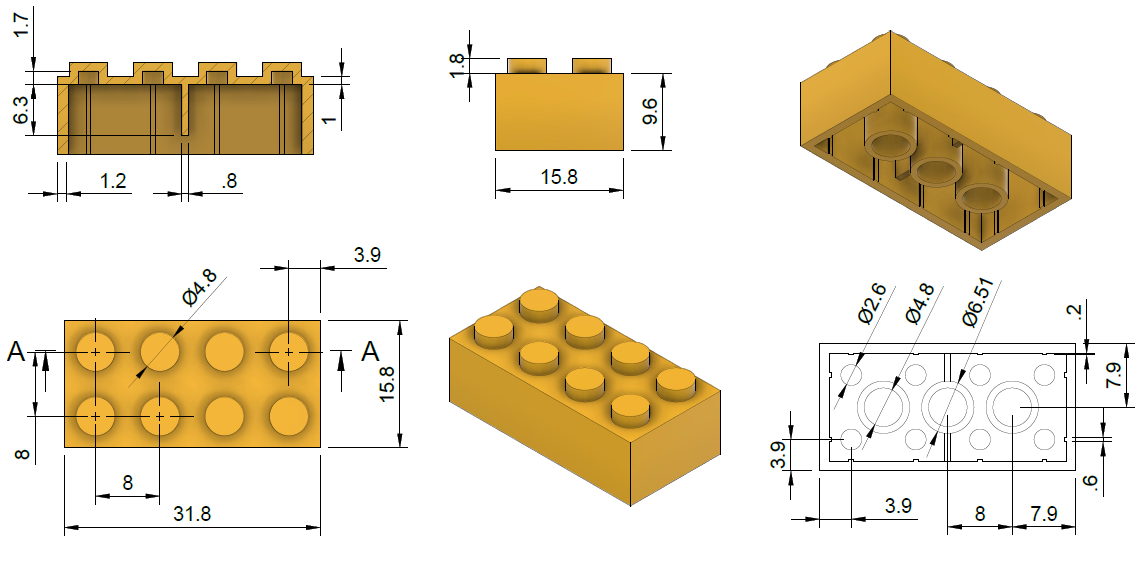
\includegraphics[width=0.8\columnwidth]{fig/LEGO 2x4 Brick horizontal.png}
    \caption{Maße des Standard 2x4 LEGO Steins \cite{LEGOBric2:online}}
    \label{fig:Lego 2x4 Brick}
\end{figure}

\section{Mauerwerksbau}
\label{basics: Mauerwerksbau}
Der Mauerwerksbau ist eine Art des Massivbaus, bei welchem Natur- oder Formsteine aufgeschichtet werden, um Wände beziehungsweise Mauern zu errichten.
Eine derart gebaute Wand besteht demnach aus Steinen und den dazwischen entstehenden Fugen.
Mörtel ist dabei nicht zwangsläufig notwendig.
Man spricht von trocken versetzten Steinen oder einer Trockenmauer, wenn darauf verzichtet wird.
Heutzutage wird fast ausschließlich mit quaderförmigen Formsteinen gebaut.
Zur Beschreibung solcher Formsteine existieren zwei relevante Größen.
Die eine ist das sogenannte \textit{Baunennmaß}, mit dem die tatsächliche Größe des Steins angegeben wird.
Die andere das \textit{Baurichtmaß}, das sich aus Baunennmaß und dem Fugenmaß zusammensetzt.
Baurichtmaße sind gemäß dem oktametrischen Maßsystem immer ein Vielfaches von \(12,5 cm\) (das entspricht \(1/8 m\)) und mindestens \(6.25cm\).
Dies gilt sowohl für die Breite als auch die Höhe der Steine.
Das System ist in der DIN 4172 Maßordnung im Hochbau geregelt und ist das fest definierte Grundmaß für das Bauwesen in Europa\cite{DIN417224}.

\begin{figure}[ht]
    \centering
    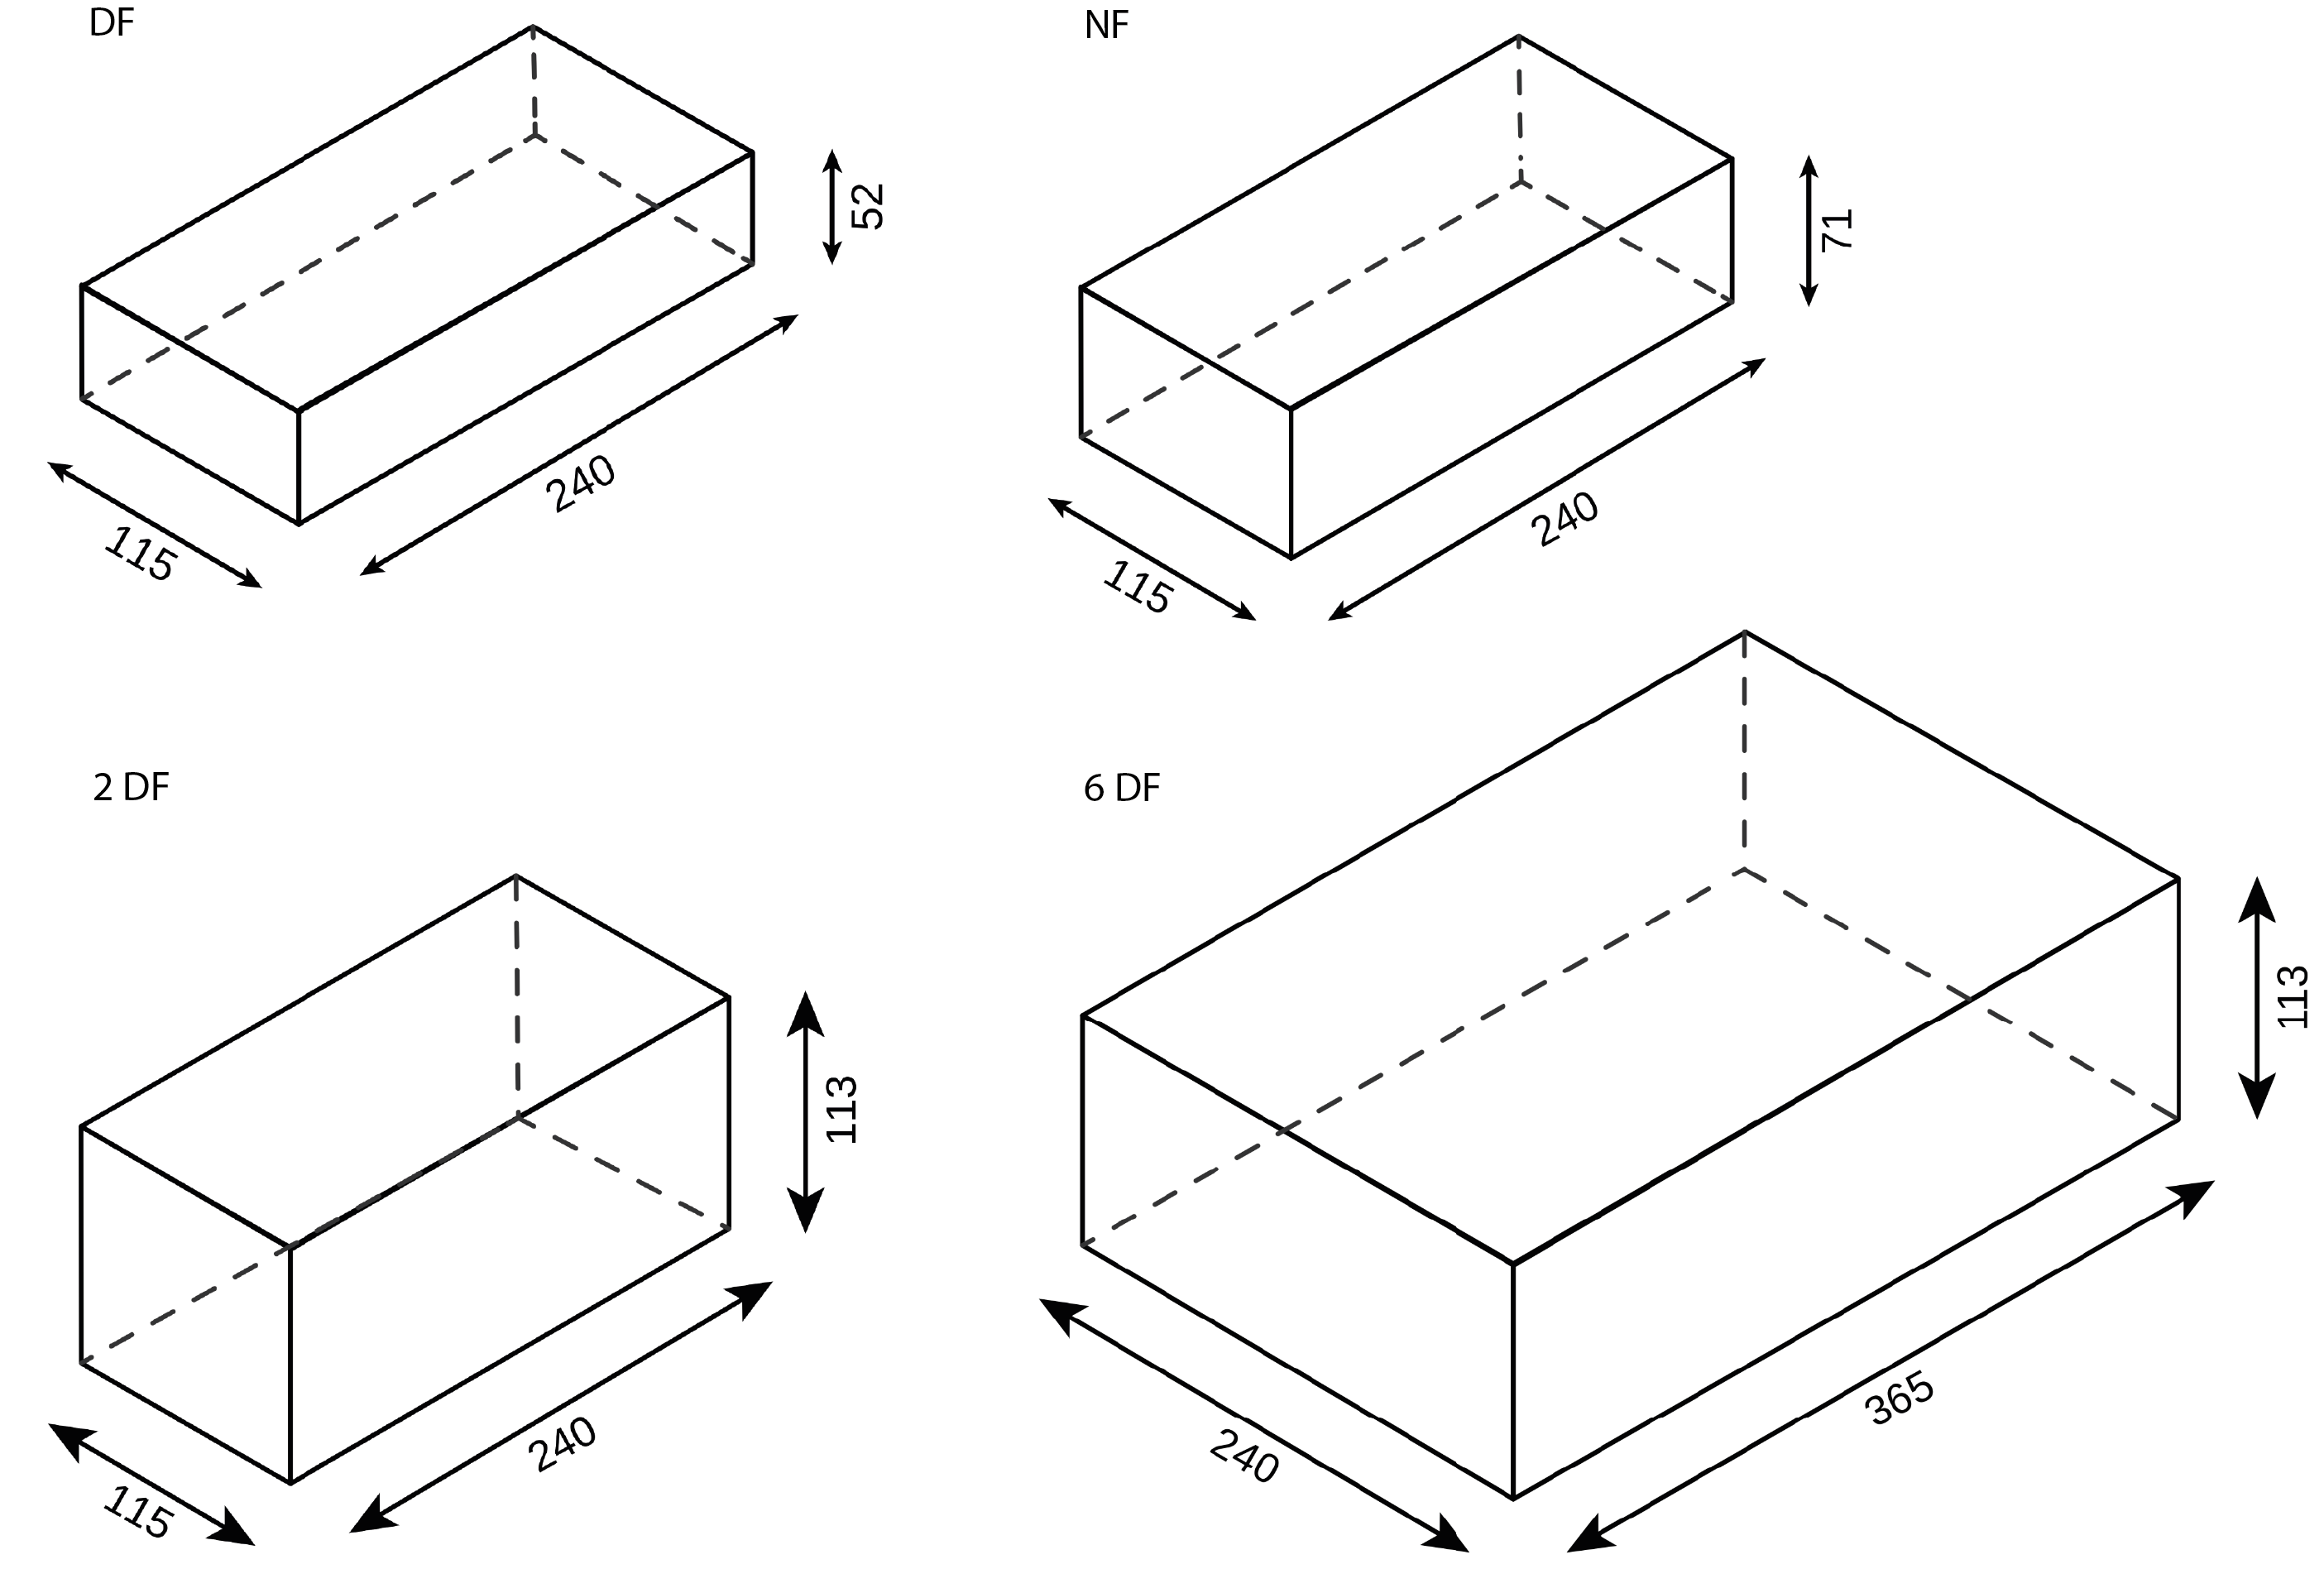
\includegraphics[width=0.8\columnwidth]{fig/Ziegelsteinformate DF NF 2DF 6DF.png}
    \caption{Darstellung verschiedener Steinformate nach DIN 4172 (Baunennmaß in Millimetern) \cite{Steinfor38:online}}
    \label{fig:Steinformate}
\end{figure}

Daraus gehen insbesondere folgende zwei Formate für Ziegelsteine hervor:
Das Normalformat (NF) mit \(240 x 115 x 71 mm\) und das Dünnformat (DF) mit  \(240 x 115 x 52 mm\) (Länge x Breite x Höhe).
Alle anderen Formate werden mithilfe dieser beiden Grundsteine angegeben.
So sind zum Beispiel die in Abbildung \ref{fig:Steinformate} gezeigten 2 DF und 6 DF Steine eine Kombination aus mehreren Steinen im Dünnformat.
Dabei sieht die Norm ein Fugenmaß von \(1 cm\) für Stoßfugen (vertikal) und \(1.2 cm\) for Lagerfugen (horizontal) vor.
Für Systeme, die eine schmalere oder keine Fuge benötigen, werden entsprechend größere Steine hergestellt, um der Maßordnung zu entsprechen.
Mithilfe des Systems ist man zusätzlich in der Lage Türen und Fenster an die daraus entstehenden Öffnungen anzupassen und vermeidet zeitaufwendiges, nachträgliches Anpassen.

\subsection{Mauerwerksverband}
\label{basics:Mauerwerksverband}
Als Mauerwerksverband bezeichnet man bestimmte, gleichmäßige Anordnungen von Mauersteinen, um einen homogenen Mauerwerkskörper zu erreichen \cite{Mauerwer39:online}.
Damit kann eine gleichmäßige Kraftverteilung innerhalb der Mauer gewährleistet werden.
Eine wichtige Rolle nimmt dabei das Überbindemaß ein, welches die Mindestüberlappung von Mauersteinen aus zwei Schichten der Mauer vorgibt.
Für das planmäßige Überbindemaß \(l_{ ol }\) gilt für übliche Mauersteine mit Schichthöhen \(h_{ u } \leq 249 mm\) nach DIN EN 1996-1-1: \( l_{ ol } \geq 0,4 · h_{ u } \geq 45 mm\)\cite{Bemessun72:online}\cite{DIN_EN_1996_1_1}.
Zudem wird darin die Mindestwanddicke für tragendes Mauerwerk, "sofern aus Gründen der Standsicherheit, der Bauphysik oder des Brandschutzes nicht größere Dicken erforderlich sind" \cite{Bemessun72:online}, auf  \(t_{ min } = 115 mm\) festgelegt \cite{DIN_EN_1996_1_1}.
Dies ist, wie in Abbildung \ref{fig:Steinformate} zu sehen, exakt die Breite der kleinsten Ziegelformate NF und DF.

Man unterscheidet zwei Arten von Mauerwerk: das Einsteinmauerwerk und das Verbandsmauerwerk.
Wie schon dem Namen zu entnehmen, handelt es sich beim Einsteinmauerwerk und ein Mauerwerk, bei welchem die Wanddicke der Steindicke entspricht.
Hier muss das Überbindemaß lediglich über die Wandlängsrichtung eingehalten werden.
Bei Verbandsmauerwerk gilt dies zusätzlich für die Wandquerrichtung. \cite{05maurer1:online}

\begin{figure}[htb]
  \begin{subfigure}[b]{0.5\columnwidth}
    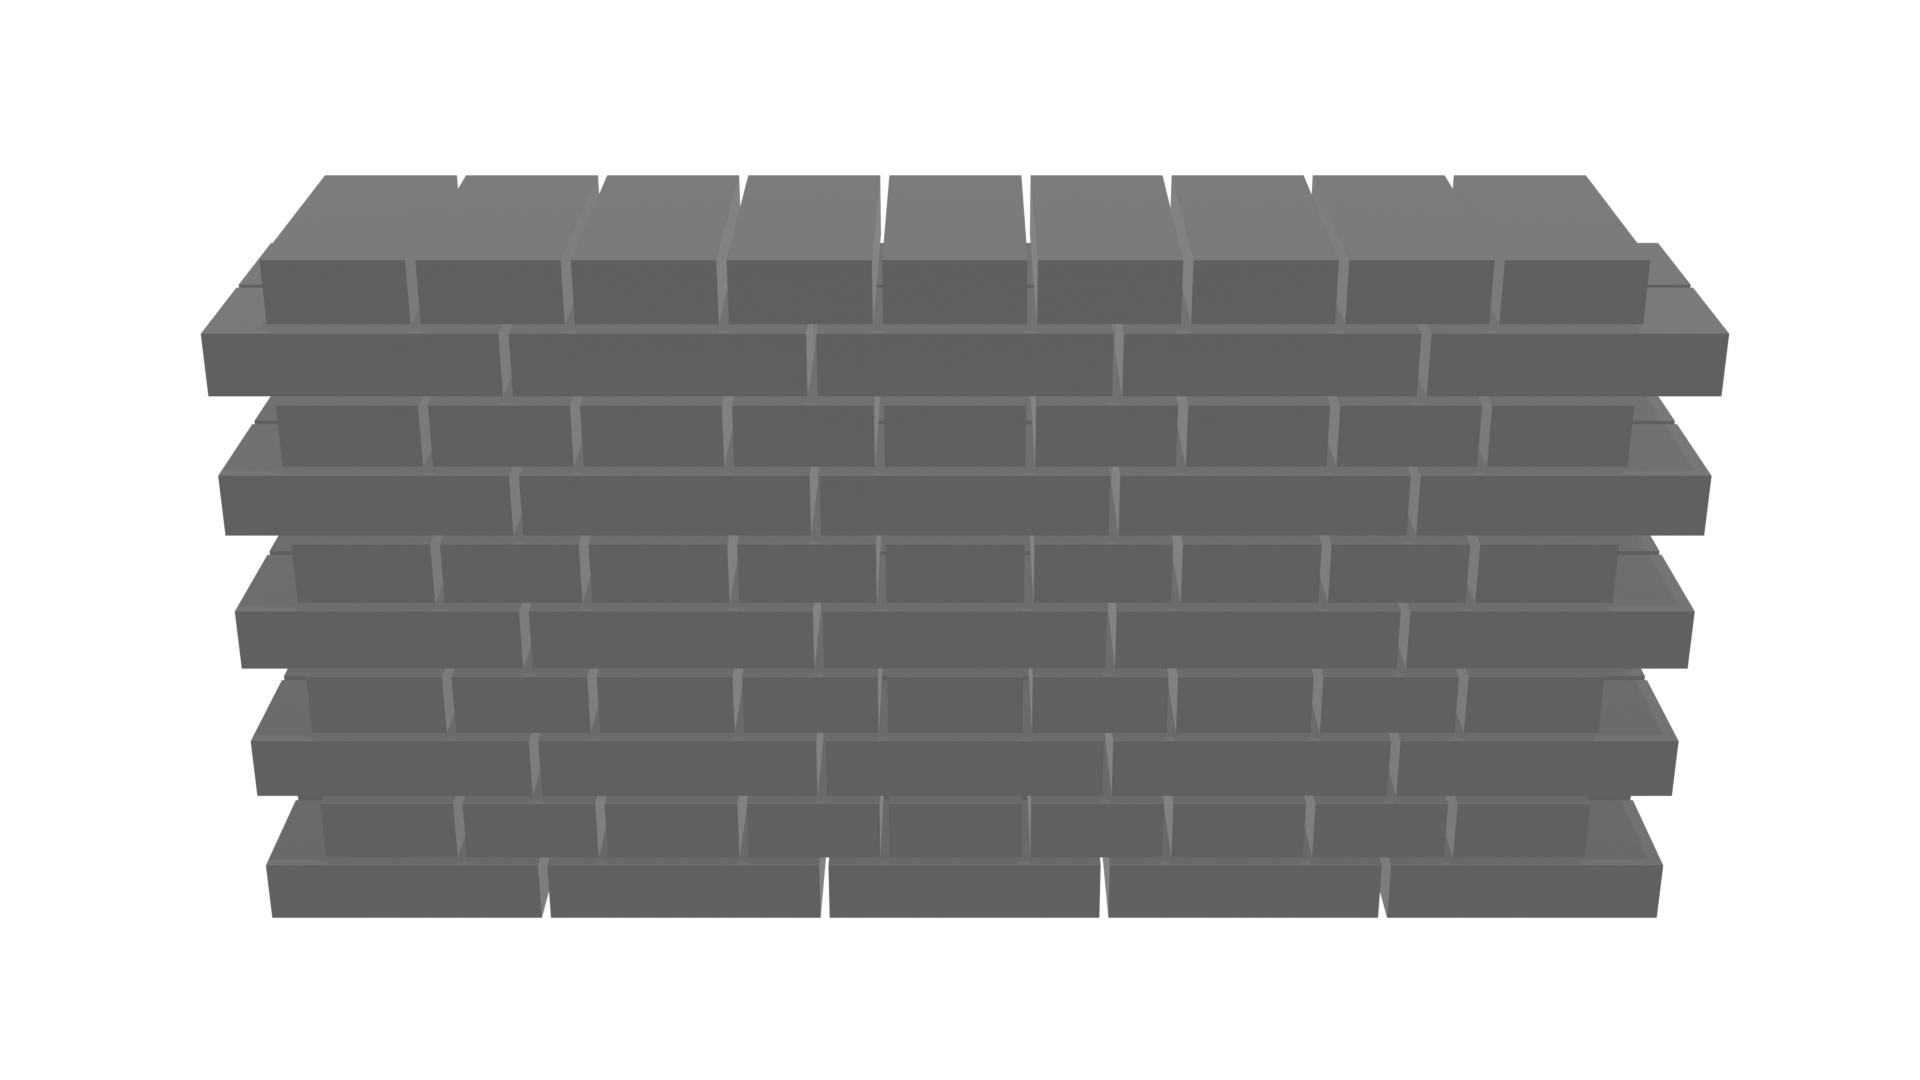
\includegraphics[width=\columnwidth]{fig/blockverband.png}
    \caption{Blockverband.}
    \label{fig:basics:blockverband}
  \end{subfigure}
  \hfill
  \begin{subfigure}[b]{0.5\columnwidth}
    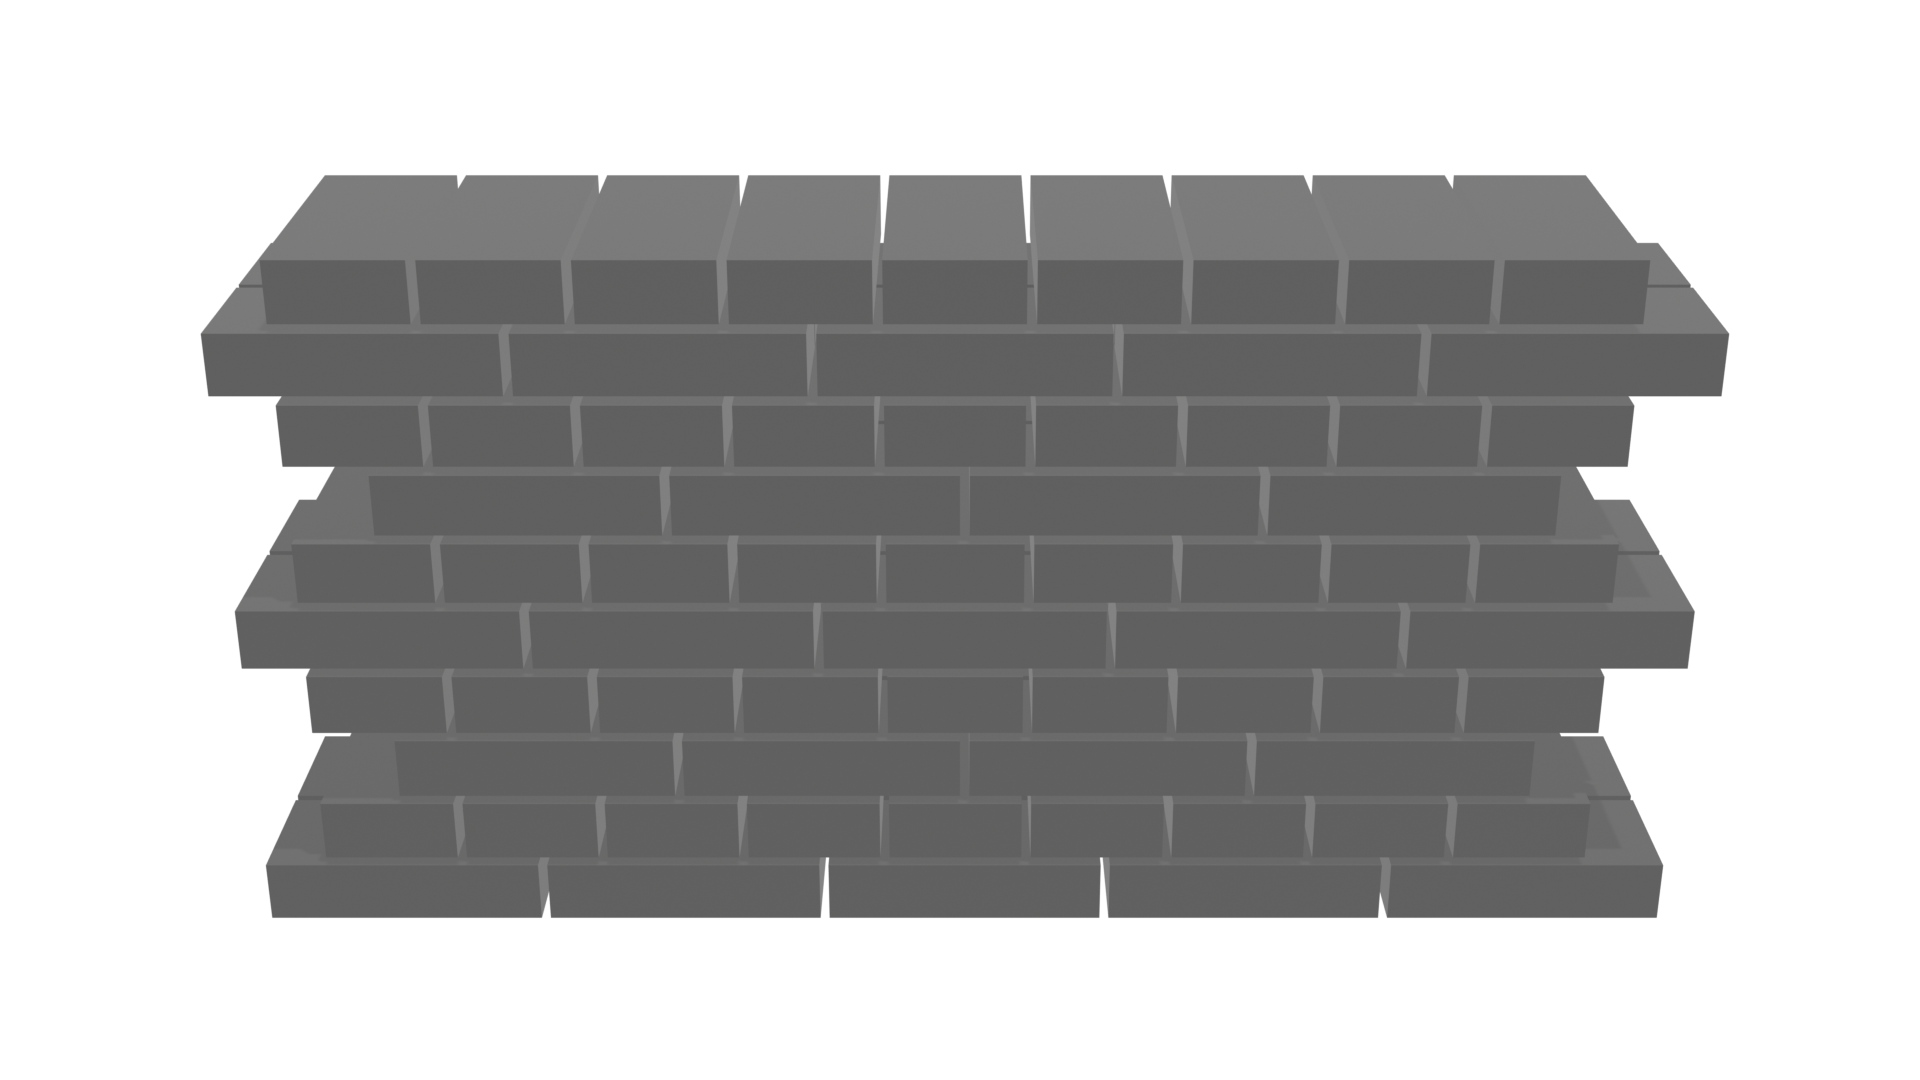
\includegraphics[width=\columnwidth]{fig/kreuzverband.png}
    \caption{Kreuzverband.}
    \label{fig:basics:kreuzverband}
  \end{subfigure}
  \begin{subfigure}[b]{0.5\columnwidth}
    \includegraphics[width=\columnwidth]{fig/läuferverband025_mittig.png}
    \caption{Mittlerer Läuferverband \textit{(Versatz: 1/4 der Steinlänge).}}
    \label{fig:basics:läuferverband_mittig}
  \end{subfigure}
  \begin{subfigure}[b]{0.5\columnwidth}
    \includegraphics[width=\columnwidth]{fig/läuferverband033_schleppend.png}
    \caption{Schleppender Läuferverband \textit{(Versatz: 1/3 der Steinlänge).}}
    \label{fig:basics:läuferverband_schleppend}
  \end{subfigure}
  \begin{subfigure}[b]{0.5\columnwidth}
    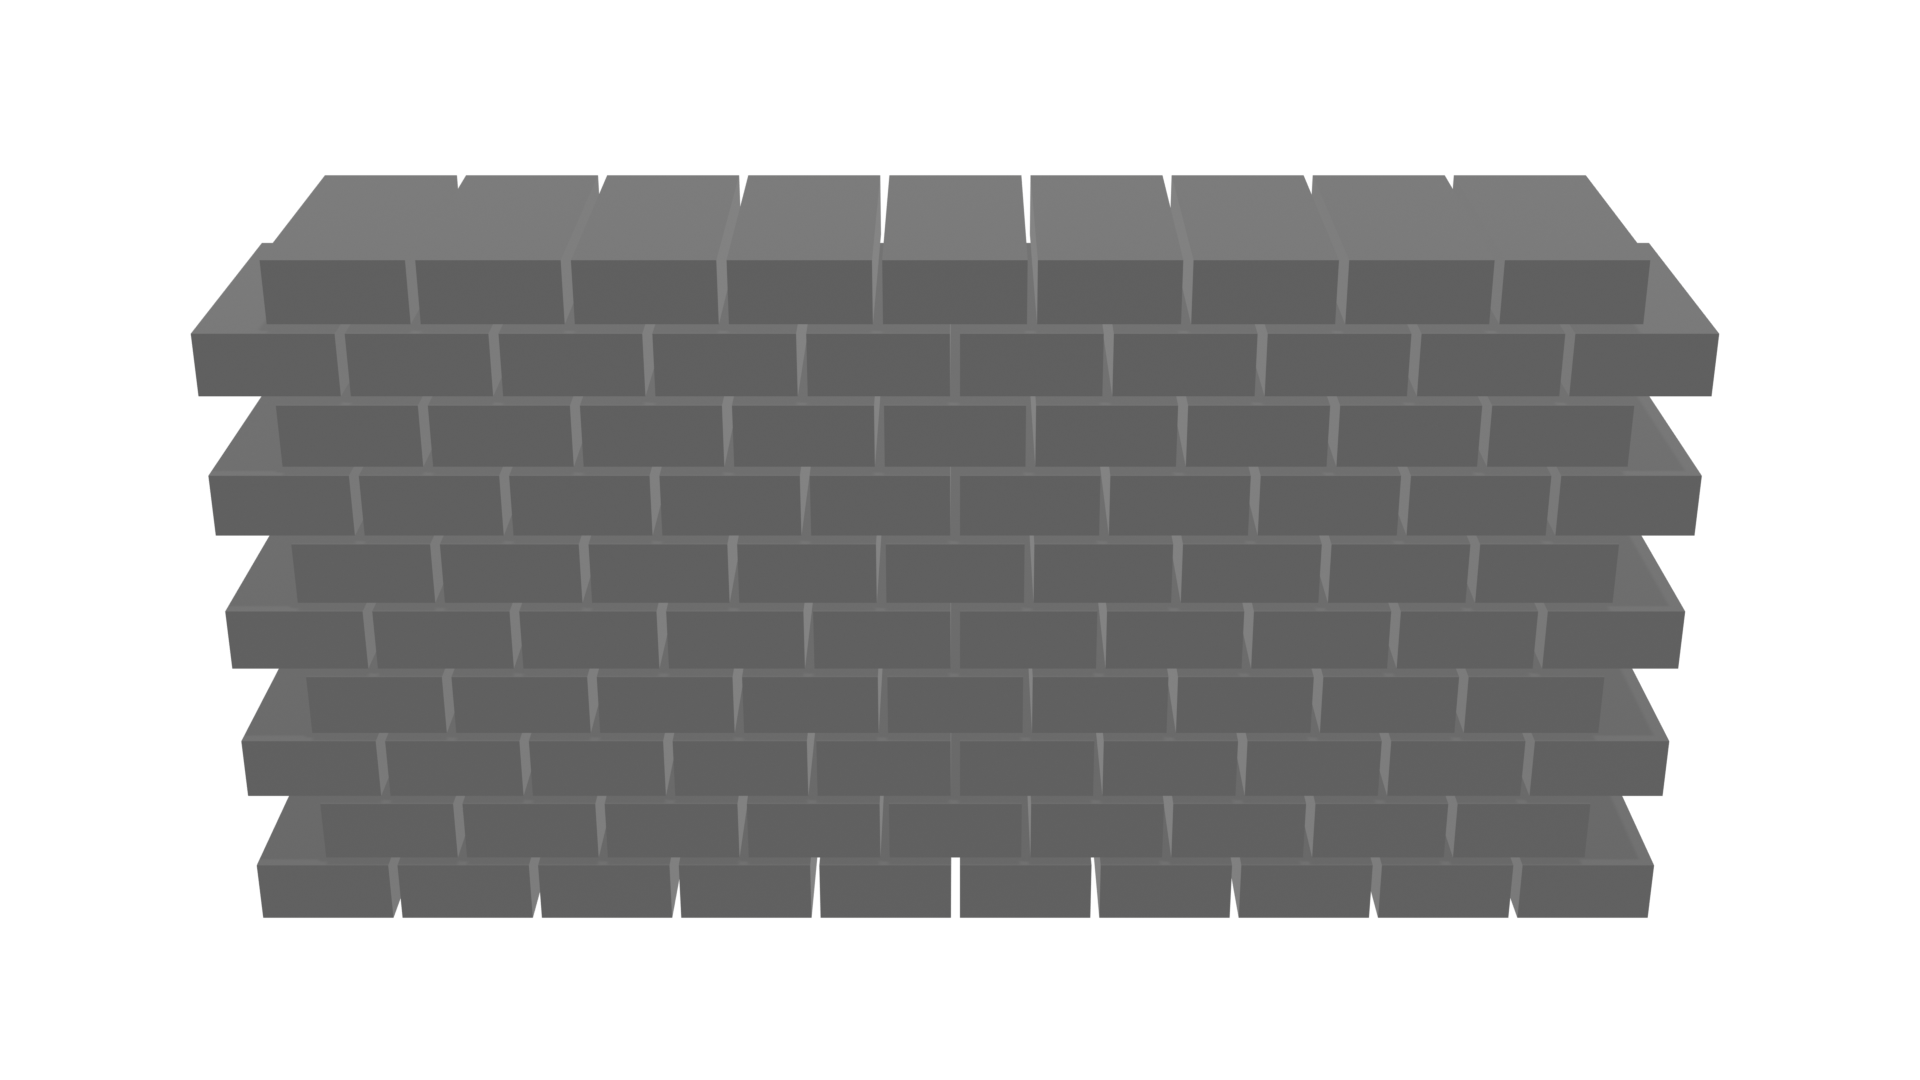
\includegraphics[width=\columnwidth]{fig/kopfverband.png}
    \caption{Kopf/Binderverband.}
    \label{fig:basics:läuferverband_mittig}
  \end{subfigure}
  \begin{subfigure}[b]{0.5\columnwidth}
    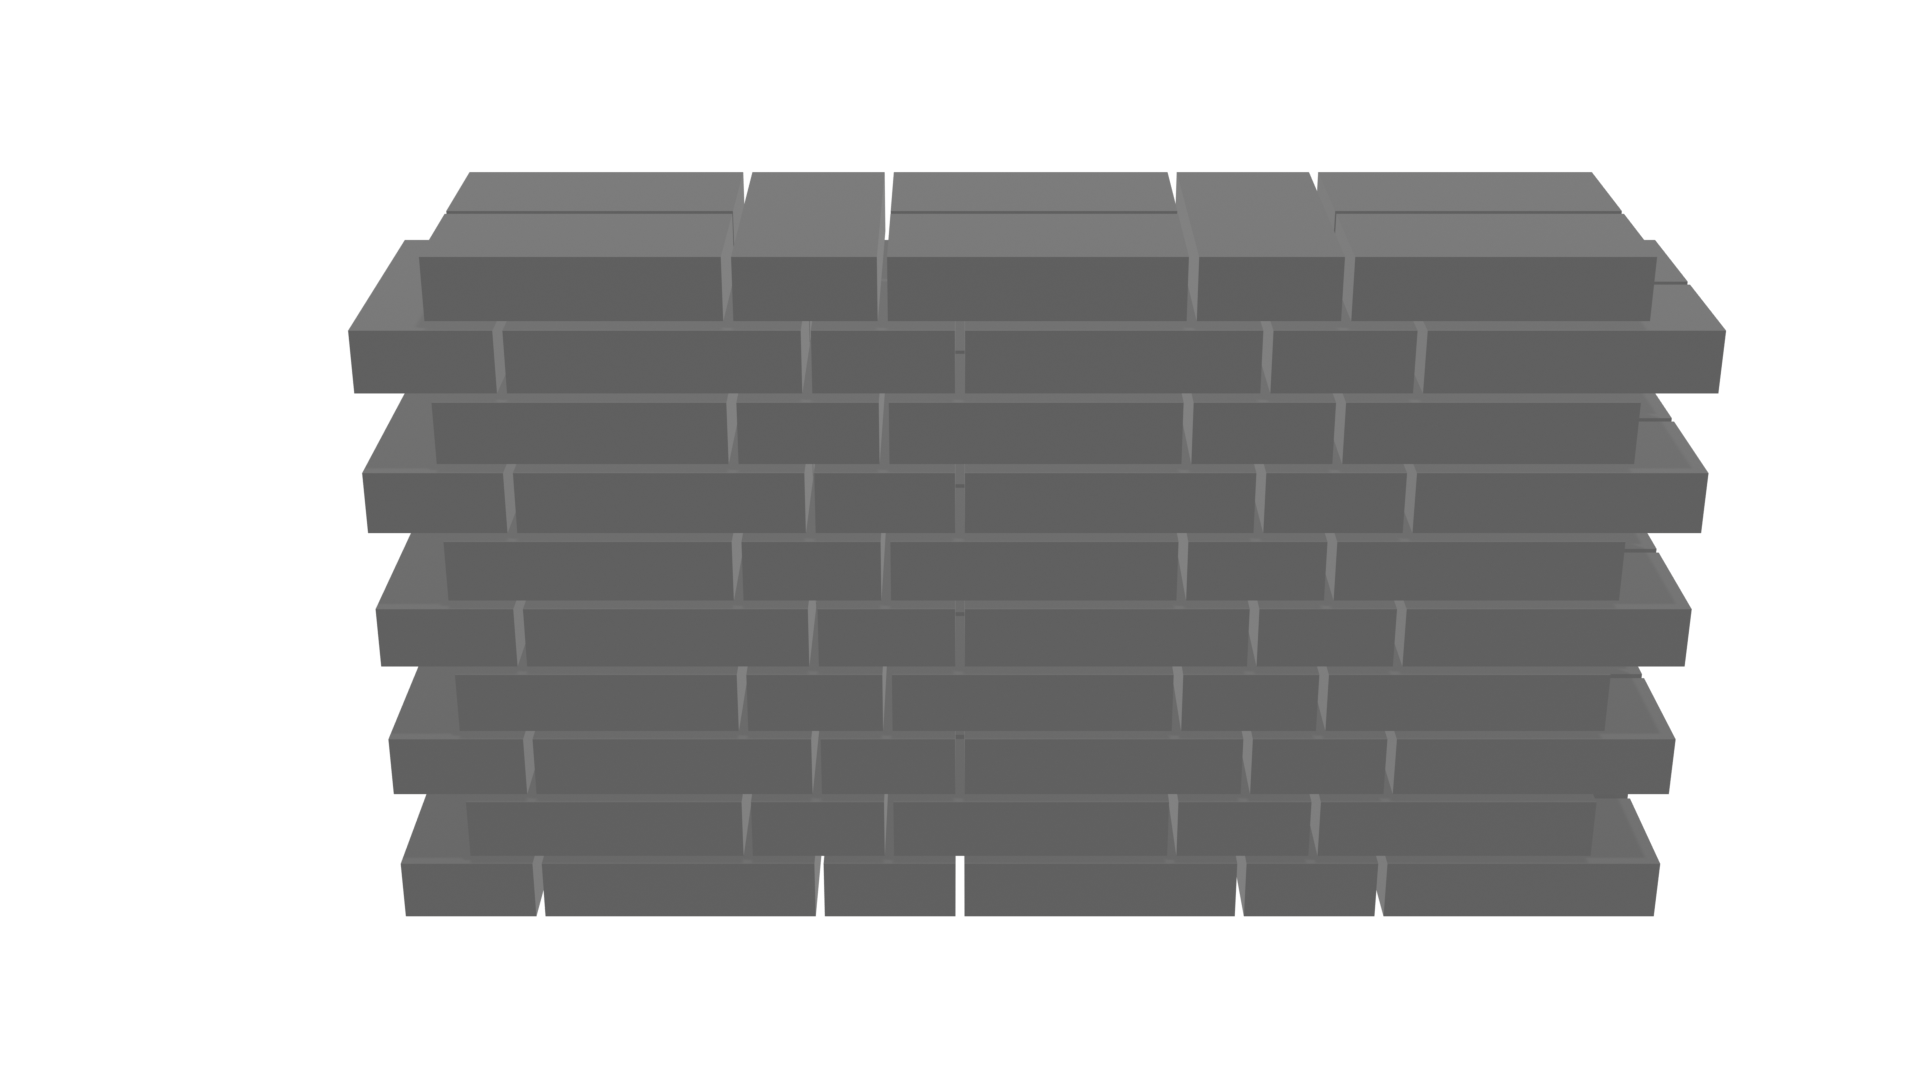
\includegraphics[width=\columnwidth]{fig/gotischerverband.png}
    \caption{Gotischer Verband.}
    \label{fig:basics:läuferverband_schleppend}
  \end{subfigure}
  \label{fig:verbände}
  \caption{Typische Mauerwerksverbände.}
\end{figure}

Treffen zwei oder mehrere Wandstücke aufeinander, so gilt es diese miteinander zu verzahnen.
Dabei muss nach wie vor das Überbindemaß eingehalten werden.
Es treten verschiedene Fälle ein: TODO Bilder!
\paragraph{Ecken}
Zwei Wandenden stehen in einem (meistens rechten) Winkel zueinander und bilden so eine Ecke.
\paragraph{Kreuzungen}
Zwei Wandenden treffen von beiden Seiten einer dritten Wand an der selben Stelle aufeinander und bilden zusammen eine Kreuzung.
Dabei ist es möglich, dass die aufeinandertreffenden Wände jeweils unterschiedliche Dicken aufweisen.
\paragraph{T-Kreuzungen}
Ein Wandende steht senkrecht auf einer anderen Wand und bildet damit eine T-Kreuzung.
Auch hier kann es vorkommen, dass die beiden Wandstücke unterschiedliche Dicken haben.
Sowohl bei Kreuzungen als auch T-Kreuzungen kann auf das aufwendige Verahnen verzichtet und stattdessen die sogenannte Stumpfstoßtechnik angewandt werden.
Dabei werden Stahlanker zwischen der Wand und den darauf treffenden "stumpfen" Wandenden verwendet, um die beiden Wände sicher miteinander zu verbinden.
\paragraph{Wandenden}
Eine Wandende steht frei im Raum, ohne ein anderes Wandstück zu berühren. 
Dafür muss der verwendete Mauerwerksverband zu einem geraden Abschluss gebracht werden.
Öffnungen innerhalb eines Wandstücks können in der selben Art behandelt werden, da der vorherrschende Verband in den betroffenen Schichten gerade unterbrochen werden muss.
Über Öffnungen für Fenster und Türen wird ein sogenannter Sturz gelegt, welcher ebenfalls in den der Wand zugrunde liegenden Mauerwerksverband eingebunden werden muss.

Die Lösungen für die oben geannten Situationen variieren je nach angestrebten Mauerwerksverband und der verwendeten Modulgröße stark. 
Gleichzeitig beeinflussen unterschiedliche Ecklösungen die Art in der ein Wandende gemauert werden muss.
TODO Bild von ecklösung und kreuzung für läuferverband und einem größerem verband:\label{basics:mauerwerk_eckloesung}
% https://www.ks-maurerfibel.de/maurerfibel/4-mauerwerksverbaende/4-4-einsteinmauerwerk-eckloesungen/
% https://www.ks-maurerfibel.de/maurerfibel/4-mauerwerksverbaende/4-5-verbandsmauerwerk-eckloesungen/
% https://www.ks-maurerfibel.de/maurerfibel/4-mauerwerksverbaende/4-7-mauern-von-stoessen-und-kreuzungen/

%https://baulexikon.beuth.de/MAUERWERKSVERBAND.HTM
%https://www.bauprofessor.de/mauerwerksverband/
DIN 1053-1 (wurde durch DIN EN 1996-1-1 ersetzt)
anstoßendes Wandstück: der bereich an dem zwei wandsegmente aneinanderstoßen z.b eine ecke
%https://www.baunetzwissen.de/mauerwerk/fachwissen/planungsgrundlagen/verbaende-und-verzahnung-162752
Verzahnung: aus https://baulexikon.beuth.de/VERZAHNUNG.HTM : Verzahnung, im Mauerwerksbau übliche Technik, beim Herstellen einer Wand eine Verbindungsstelle für eine später zu errichtende und in die bereits bestehende einzubindende Wand den Verbandsregeln entsprechend vorzubereiten. Es gibt Lochverzah- nung, stehende und liegende Verzahnung. Nur die letztgenannte Verzahnungsart gilt nach DIN 1053-1 als ausreichende Verbindung zwischen tragenden und aussteifenden Mauerwerkswänden
Überbindemaß ist wichtig um Mauerwerksverbände zu bewerten
%https://www.mauerwerksbau-lehre.de/vorlesungen/1-grundlagen-und-baustoffe-des-mauerwerksbaus/13-wandkonstruktionen/132-mauerwerksverband-und-ueberbindemass

TODO Rund Wände, keine 90 Grad Ecken

\section{BRep}
\label{basics:brep}
\section{Definitionen}
\subsection{Bausteintyp}
\subsection{Baustein}
\subsection{Wand}